\section*{Problem 1}
\subsection*{Part a}
The z rotation gate is
\eq{
RZ(\theta) &= \begin{pmatrix}
    e^{-i\frac{\theta}{2}} & 0\\
    0 & e^{i\frac{\theta}{2}}\\
    \end{pmatrix}\\
    &= e^{-i\frac{\theta}{2}}
    \begin{pmatrix}
    1 & 0\\
    0 & e^{i\theta}
    \end{pmatrix}\\
\implies RZ(\frac{\pi}{4}) &= e^{-i\frac{\pi}{8}}
\begin{pmatrix}
1 & 0\\
0 & e^{i\frac{\pi}{4}}
\end{pmatrix}\\
&= e^{-i\frac{\pi}{8}} \hat{T}
}
\subsection*{Part b}
The gate sequence matrix is
\eq{
\hat{H}\hat{T}\hat{H} &= 1/2
\begin{pmatrix}
    1 + e^{i\frac{\pi}{4}} & 1 - e^{i\frac{\pi}{4}}\\
    1 - e^{i\frac{\pi}{4}} & 1 + e^{i\frac{\pi}{4}}
\end{pmatrix}\\
&= 1/2 (\sigma_0 (1 + e^{i\frac{\pi}{4}})+\sigma_x(1 - e^{i\frac{\pi}{4}}))\\
&= 1/2 e^{i\frac{\pi}{8}} (\sigma_0 (e^{-i\frac{\pi}{8}} + e^{i\frac{\pi}{8}})-\sigma_x(e^{i\frac{\pi}{8}} - e^{-i\frac{\pi}{8}}))\\
&= e^{i\frac{\pi}{8}} (\sigma_0 \cos(\frac{\pi}{8})-i\sigma_x\sin(\frac{\pi}{8}))\\
&= e^{i\frac{\pi}{8}} RX(\frac{\pi}{4})
}
\subsection*{Part c}
First we'll rewrite $\hat{H}\hat{T}\hat{H}$ and $\hat{T}$
\eq{
\hat{T} &= e^{i\frac{\pi}{8}}RZ(\frac{\pi}{4})\\
&= e^{i\frac{\pi}{8}} \begin{pmatrix}
    e^{-i\frac{\pi}{8}} & 0\\
    0 & e^{i\frac{\pi}{8}}
\end{pmatrix}\\
\hat{H}\hat{T}\hat{H}&= e^{i\frac{\pi}{8}} RX(\frac{\pi}{4})\\
&=e^{i\frac{\pi}{8}} \begin{pmatrix}
    \cos \frac{\pi}{8} & -i\sin \frac{\pi}{8}\\
    -i\sin \frac{\pi}{8} & \cos \frac{\pi}{8}
\end{pmatrix}\\
\hat{T}\hat{H}\hat{T}\hat{H} &= e^{i\frac{\pi}{4}} \begin{pmatrix}
    e^{-i\frac{\pi}{8}} & 0\\
    0 & e^{i\frac{\pi}{8}}
\end{pmatrix}
\begin{pmatrix}
    \cos \frac{\pi}{8} & -i\sin \frac{\pi}{8}\\
    -i\sin \frac{\pi}{8} & \cos \frac{\pi}{8}
\end{pmatrix}\\
&= e^{i\frac{\pi}{4}} \begin{pmatrix}
    e^{-i\frac{\pi}{8}}\cos \frac{\pi}{8} & e^{i\frac{11}{8}\pi}\sin \frac{\pi}{8}\\
    e^{i\frac{13}{8}\pi}\sin \frac{\pi}{8} & e^{i\frac{\pi}{8}}\cos \frac{\pi}{8}
\end{pmatrix}\\
&= e^{-i\frac{\pi}{4}} \begin{pmatrix}
    \cos \theta + in_z \sin \theta & i n_x \sin \theta + n_y \sin \theta\\
    in_x \sin \theta -n_y \sin \theta & \cos \theta -in_z \sin \theta
\end{pmatrix}
}
With some algebra we deduce that
\eq{
\theta &= \arccos (\cos^2 \frac{\pi}{8})\\
n_x &= -\frac{\sin \frac{\pi}{8}\cos \frac{\pi}{8}}{\sin \theta}\\
n_y &= -\frac{\sin^2 \frac{\pi}{8}}{\sin \theta}\\
n_z &= -\frac{\sin \frac{\pi}{8}\cos \frac{\pi}{8}}{\sin \theta}\\
}
Letting $\hat{n} = (n_x,n_y,n_z)$ we can write
\eq{
\hat{T}\hat{H}\hat{T}\hat{H} &= e^{i\frac{\pi}{4}} e^{i \theta \hat{n}\cdot \Vec{\sigma}}\\
&= e^{i\frac{\pi}{4}} e^{-\frac{i}{2} \phi \hat{n}\cdot \Vec{\sigma}}
}
So the angle of rotation is then
\eq{
\phi &= -2\arccos (\cos^2 \frac{\pi}{8})
}
\subsection*{Part d}
We can't produce any rotation on the Bloch sphere, but we can prove that any rotation about the axis defined by $\hat{n}$ can be achieved in the limit of an infinite number of gates.

First we do a change of variables from $\theta \rightarrow \gamma$, where we're effectively going from $\mathbb{R}/2\pi \mathbb{Z}\rightarrow \mathbb{R}/\mathbb{Z}$.
\eq{
\theta &= \frac{\gamma}{2\pi}
}
The rotation of the operator applied $k$ times is
\eq{
\gamma_k &= 2\pi \theta_k\\
&= k \arccos(\cos^2 \frac{\pi}{8})
}
Since $\theta_1$ is irrational, by the equidistribution theorem, the sequence $\gamma_1, \gamma_2, \gamma_3 \dots$ is uniformly distributed on $\mathbb{R}/\mathbb{Z}$. Pick some arbitrary rotation $\psi \in [0,1]$ and a small $\epsilon = \frac{1}{2n}$. Then in the large $n$ limit, the number of $\gamma_i$ in the region $[\psi -\epsilon, \psi + \epsilon]$ approaches $2\epsilon n = 1$.

To approximate an arbitrary rotation exactly we would need an infinite number of rotations.

\pagebreak
\section*{Problem 2}
\subsection*{Part a}
The starting state is
\eq{
\ket{\phi_{init}} &= \ket{\psi} \otimes \frac{1}{\sqrt{2}}(\ket{00} + \ket{11})\\
\ket{\phi_{final}} &= \hat{CZ}^{(3)}\hat{CX}^{(3)}\hat{H}^{(1)}CNOT^{(2)}\ket{\phi_{init}}\\
}
If $\ket{\psi} = \ket{0}$
\eq{
\ket{\phi_{final}} &= \hat{CZ}^{(3)}\hat{CX}^{(3)}\hat{H}^{(1)}\ket{0} \otimes \frac{1}{\sqrt{2}}(\ket{00} + \ket{11})\\
&= \hat{CZ}^{(3)}\hat{CX}^{(3)}\frac{1}{2}(\ket{1}-\ket{0}) \otimes (\ket{00} + \ket{11})\\
&= \frac{1}{2}(\ket{100}-\ket{110} -\ket{000} + \ket{010})
}
So the 3rd qubit is in state $\ket{0}$, similarly if $\ket{\psi} = \ket{1}$ then the 3rd qubit is in state $\ket{1}$.
\subsection*{Part b}
The quantum circuit generated is below, the code is in the appendix\footnote{X and Z are controlled gates but QuTip doesn't seem to draw these wires from classical bits.}.
\begin{figure}[H]
    \centering
    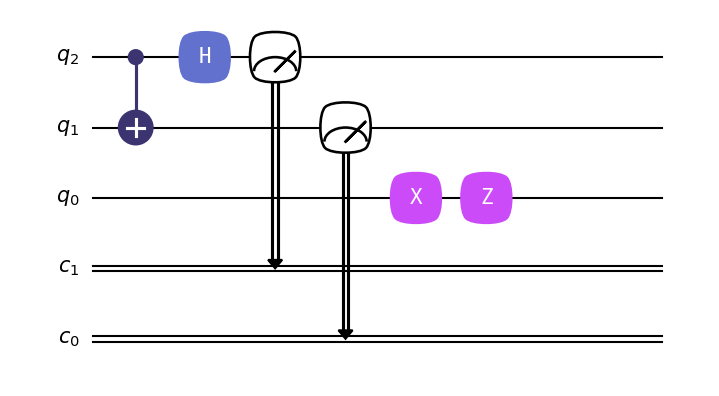
\includegraphics[width=1\linewidth]{Resources//245//Homework 8/245 Homework 8 Problem 2b.png}
    \caption{Quantum teleportation circuit, generated in QuTip.}
\end{figure}
The output of the above circuit for $q_0$ as a function of initial states $\ket{0}$ and $\ket{1}$ are, respectively,
$$\left(\begin{array}{cc}1\\0\\0\\0\\0\\0\\0\\0\end{array}\right) = \ket{0} \textrm{ and }\left(\begin{array}{cc}0\\0\\0\\0\\1\\0\\0\\0\end{array}\right) = \ket{1}$$
\pagebreak
\section*{Problem 3}
We can construct a two bit half adder using two controlled not gates and a Toffoli gate.\\
\begin{figure}[H]
\centering
\begin{quantikz}
\lstick{$\ket{\psi_1}$} & \ctrl{2} &  & \ctrl{3} &\\
\lstick{$\ket{\psi_2}$} & \control{} & \ctrl{2}  & &\\
\lstick{$\ket{0}$} & \targ{} & & &\\
\lstick{$\ket{0}$} & & \targ{} & \targ{}&\\
\end{quantikz}
\caption{Quantum two-bit half adder.}
\end{figure}
This circuit operates by first flipping the carry digit if both inputs are up, if both inputs are up then the add digit is flipped twice -effectively leaving it at $0$. If only one qubit is up then nothing happens to the carry digit and the add digit is flipped once.

\begin{table}[H]
    \centering
    \begin{tabular}{ccccc}
        \ket{\psi_1 \psi_2} & \ket{00} & \ket{01} & \ket{10} & \ket{11}\\
        \ket{\phi_1 \phi_2} & \ket{00} & \ket{01} & \ket{01} & \ket{10}\\
    \end{tabular}
    \caption{Quantum two-bit half adder truth table.}
    \label{tab:my_label}
\end{table}
The code to verify this circuit is in the appendix.
\pagebreak
\section*{Problem 4}
\subsection*{Part a}
We have
\eq{
\hat{D}\hat{O}\ket{s} &= \cos \theta \hat{D}\hat{O} \ket{s'} + \sin \theta \hat{D} \hat{O} \ket{q}\\
&= \cos \theta \hat{D} \ket{s'} -\sin \theta \hat{D} \ket{q}\\
&= \cos (\theta) 2 \ket{s}\braket{s | s'}-\cos \theta \ket{s'} - \sin (\theta) 2\ket{s} \braket{s | q} + \sin \theta \ket{q}\\
}
We now have to compute the outer products
\eq{
\ket{s}\braket{s | s'} &= (\cos \theta \ket{s'} + \sin \theta \ket{q})(\bra{s'} \cos \theta + \bra{q} \sin \theta)\ket{s'}\\
&= (\cos \theta \ket{s'} + \sin \theta \ket{q})\cos \theta\\
&= \cos^2 \theta \ket{s'}+\cos \theta \sin \theta \ket{q}\\
\ket{s}\braket{s | q} &= (\cos \theta \ket{s'} + \sin \theta \ket{q})(\bra{s'} \cos \theta + \bra{q} \sin \theta)\ket{q}\\
&= (\cos \theta \ket{s'} + \sin \theta \ket{q})\sin \theta\\
&= \cos \theta \sin \theta \ket{s'}+\sin^2 \theta \ket{q}
}
Substituting back in
\eq{
\hat{D}\hat{O}\ket{s} &=2\cos^3 \theta \ket{s'}+2\cos^2 \theta \sin \theta \ket{q} -\cos \theta \ket{s'}\\
& - 2\cos \theta \sin^2 \theta \ket{s'}-2 \sin^3 \theta \ket{q} +\sin \theta \ket{q}\\
& = (2\cos^3 \theta -2\cos \theta \sin^2 \theta -\cos \theta )\ket{s'}\\
& + (-2 \sin^3 \theta + 2 \cos^2 \theta \sin \theta + \sin \theta)\ket{q}\\
& = \cos \theta (2\cos^2 \theta -2\sin^2 \theta -1 )\ket{s'}\\
& + \sin \theta (-2 \sin^2 \theta + 2 \cos^2 \theta + 1)\ket{q}\\
& = \cos \theta (2\cos 2 \theta -1 )\ket{s'}\\
& + \sin \theta (2\cos 2\theta + 1)\ket{q}\\
&= \cos 3 \theta \ket{s'} + \sin 3 \theta \ket{q}
}

\subsection*{Part b}
The probability is
\eq{
\mathbb{P} &= |\braket{q|\hat{D}\hat{O}|s}|^2\\
&= |\sin 3 \theta |^2\\
&= \sin^2 3 \theta\\
&= (3\sin \theta - 4 \sin^3 \theta )^2
}
We now have to find $\sin \theta$
\eq{
\braket{q|s} &= \sin \theta\\
&= \bra{q} \frac{1}{\sqrt{N}}\sum_{i = 0}^{N-1}\ket{x}\\
&= \frac{1}{2}
}
So it follows that
\eq{
\mathbb{P} &= (\frac{3}{2}-\frac{4}{8})^2\\
 &= 1
}
\pagebreak
\section*{Appendix}
\subsection*{Problem 2}
\begin{python}
from qutip_qip.operations import Measurement
from qutip_qip.circuit import QubitCircuit
from qutip import ket, tensor
from numpy import sqrt

teleportation = QubitCircuit(3, num_cbits=2, reverse_states=True)

teleportation.add_gate("CNOT", controls=[2], targets=[1])
teleportation.add_gate("H", controls=None, targets=[2])

teleportation.add_measurement("M0", targets=[2], classical_store=1)
teleportation.add_measurement("M1", targets=[1], classical_store=0)

teleportation.add_gate("X", targets=[0], classical_controls=[0])
teleportation.add_gate("Z", targets=[0], classical_controls=[1])

def teleport(psi_starting):
    bell_state = 1/sqrt(2)*(ket("00") + ket("11"))
    starting_state = tensor(psi_starting, bell_state)
    
    final_state = teleportation.run(starting_state)
    final_measurement = Measurement("Psi", targets = [0])
    return final_measurement.measurement_comp_basis(final_state)

display(teleportation)
display(teleport(ket("0")))
display(teleport(ket("1")))
\end{python}

\pagebreak
\subsection*{Problem 3}
\begin{python}
from qutip_qip.operations import (toffoli, cnot, gate_sequence_product, Measurement)
from qutip_qip.circuit import QubitCircuit
from qutip import ket, basis


q = QubitCircuit(4, reverse_states=False)

q.add_gate("TOFFOLI", controls=[3, 2], targets=[1])
q.add_gate("CNOT",controls=[3],targets=[0])
q.add_gate("CNOT",controls=[2],targets=[0])

add = Measurement("Add", targets = [0])
carry = Measurement("Carry", targets = [1])

initial_state = ket("0010")
final_state = q.run(initial_state)

print("Carry Bit: " + str(carry.measurement_comp_basis(final_state)[1][1]))
print("Add Bit: " + str(add.measurement_comp_basis(final_state)[1][1]))

q
\end{python}